\documentclass{standalone}
\usepackage{tikz}
\usepackage{ctex,siunitx}
\setCJKmainfont{Noto Serif CJK SC}
\usepackage{tkz-euclide}
\usepackage{amsmath}
\usetikzlibrary{patterns, calc}
\usetikzlibrary {decorations.pathmorphing, decorations.pathreplacing, decorations.shapes}
\pgfdeclareverticalshading{pile}{100bp}{
  color(0bp)=(black);color(50bp)=(white);color(100bp)=(black)
}
\pgfdeclareverticalshading{pile2}{100bp}{
  color(0bp)=(white);color(50bp)=(black);color(100bp)=(white)
}
\begin{document}
\small
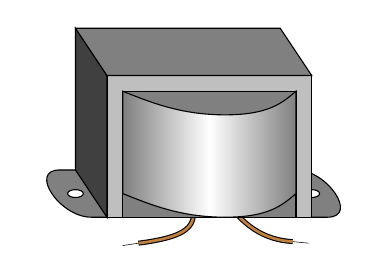
\begin{tikzpicture}[>=latex, scale=1]
  % \useasboundingbox(0.9,0)rectangle(5.1,5);
  \draw[fill=gray,even odd rule](-1.4,0.3)--(-1.7,0.3)..controls(-2.1,0.3)and(-1.7,-0.3)..(-1.3,-0.3)--(1.7,-0.3)..controls(2.1,-0.3)and(1.7,0.3)..(1.3,0.3)--cycle
  (-1.5,0)ellipse(0.1 and 0.05)(1.5,0)ellipse(0.1 and 0.05);
  \draw[double=brown,double distance=1pt](-0.08, 0.02)..controls( 0.10,-0.38)and( 0.00,-0.54)..(-0.70,-0.63)
  ( 0.34, 0.03)..controls( 0.60,-0.42)and( 0.91,-0.59)..( 1.26,-0.61);
  \draw[fill=lightgray](-1.1,-0.3)rectangle(1.5,1.5);
  \draw[fill=gray](-0.9,-0.3)rectangle(1.3,1.3);
  \draw[left color=gray,right color=gray,middle color=white]( 1.300, 0.00)..controls( 1.125,-0.15)and( 0.950,-0.30)..
  ( 0.400,-0.30)..controls(-0.150,-0.30)and(-0.525,-0.15)..(-0.900, 0.00)--
  (-0.900, 1.30)..controls(-0.525, 1.15)and(-0.150, 1.00)..
  ( 0.400, 1.00)..controls( 0.950, 1.00)and( 1.125, 1.15)..( 1.300, 1.30)--cycle;
  \draw[fill=darkgray](-1.1,-0.3)--(-1.1,1.5)--(-1.5,2.1)--(-1.5,0.3)--cycle;
  \draw[fill=gray](-1.1,1.5)--(-1.5,2.1)--(1.1,2.1)--(1.5,1.5)--cycle;
  \draw[very thin](-0.70,-0.63)--(-0.9,-0.66)(1.26,-0.61)--(1.46,-0.63);
\end{tikzpicture}
\end{document}